\documentclass[conference]{IEEEtran}
\IEEEoverridecommandlockouts
\usepackage{amsmath,amssymb}
\usepackage{graphicx}
\usepackage{booktabs}
\usepackage{url}
\usepackage[hidelinks]{hyperref}
\usepackage{cite}

\begin{document}

\title{How Much Does a Parity Experiment Prove?\\ Error Rates of the Rule That Accepts Benchmark Ports}

\author{\IEEEauthorblockN{Poorva Barve}
\IEEEauthorblockA{Independent researcher\\ poorvabarve@gmail.com}}

\maketitle

\begin{abstract}
Harbor, the evaluation framework behind Terminal-Bench, hosts more than eighty benchmarks ported to it through adapters. A port is accepted after a parity experiment: the same agent and model are run on the original harness and on the port, usually three times each, and the port passes if the two ranges of run scores overlap. We ask how much such an experiment proves. First, we derive the rule's error rates. With $k$ runs per side its false-alarm rate is exactly $2(k!)^2/(2k)!$, 10\% at $k=3$, and cannot be chosen; its power to detect a fixed gap falls as runs are added; and for a fixed gap its pass probability rises with noise. A pass means ``not rejected at the 10\% level'', never equivalence. Second, we re-analyse the 58 published comparisons with three runs per side under a pre-registered metric rule. The ports look close (median gap 0.7 points), but equivalence within 3 points can be shown for only 22 of them and within 5 points for 36, and the rule passes the four largest gaps, up to 15.6 points. Third, we cost the fix. An equivalence test with a stated margin needs about seven runs per side at the observed noise for a 3-point margin. Per-task outcomes, which both sides already produce, do not tighten the interval but expose task-level disagreement in half of the adapters, and a stratified-by-task test is the best calibrated detector of injected defects. We propose a five-line protocol and release the data, scripts and a verdict tool.
\end{abstract}

\begin{IEEEkeywords}
benchmark ports, agent evaluation, equivalence testing, evaluation harnesses, reproducibility
\end{IEEEkeywords}

\section{Introduction}

Two adapters in the Harbor repository illustrate the problem. For USACO the original harness scored 39.5, 40.5 and 41.0 in three runs and the Harbor port scored 45.7, 42.1 and 41.1. The ranges do not overlap, by 0.1 point, so the port fails Harbor's parity check. For RexBench the original harness scored 33.33 in every run and the port scored 16.67, 58.33 and 50.0. The ranges overlap, so the port passes, with a gap of 8.3 points between the means. The same rule gives opposite verdicts, and the comparison it rejects is the one whose data say more about closeness.

Harbor is the evaluation framework behind Terminal-Bench~\cite{terminal_bench}. Existing benchmarks are ported to it through adapters, and the maintainers' cross-benchmark comparisons and Harbor-Index leaderboard are built on the ports~\cite{harbor_adapters}. A port that drifts is a different benchmark under the same name. The contributor guide therefore requires a parity experiment and states the acceptance rule in one sentence: the two sides match if and only if their run-score ranges overlap~\cite{harbor_contributing}. The maintainers' paper words the check as the means agreeing ``within a margin consistent with their standard errors''~\cite{harbor_adapters}.

We ask how much a parity experiment proves. RQ1: what does the range-overlap rule guarantee? RQ2: what do the published parity runs establish? RQ3: what would a better check cost? We use only public data, the 84 parity files in the Harbor repository, the per-task result files the maintainers published on Hugging Face, and their paper, and we reran no benchmark. Our contributions are (1) the error rates of the overlap rule as a function of runs and noise, with a closed-form false-alarm rate; (2) an audit of every published parity comparison under a metric rule fixed before the analysis, reporting for each the smallest margin within which equivalence can be shown; (3) the cost of a better check: the runs an equivalence test needs, what per-task outcomes add, how often each test catches an injected defect, and a five-line protocol with a script that reads any parity file.\footnote{Data snapshot, scripts, pre-registration with dated amendments, per-task parsers, the number-to-script table and the verdict tool: \url{https://github.com/barveP/benchmark-port-parity}.}

We do not claim that any port is wrong (the gaps are mostly small), that anything was hidden (the maintainers published every run we used), that a comparison failing the rule is an adapter bug, or that we are first to note that agent evaluations are noisy~\cite{miller_error_bars,hardy_reliability,segato_infra_noise}.

\section{Background: Harbor parity experiments}

An adapter wraps an existing benchmark so that Harbor can run it. Before it is merged, its author runs the same agent and model on the original harness and on the port, $k$ times each with $k=3$ by default, and reports each side as mean $\pm$ sample standard error of the mean (SEM)~\cite{harbor_adapters}. The guide's matching criterion is range overlap: $\max(A) \ge \min(B)$ and $\max(B) \ge \min(A)$ for the two lists of run scores $A$ and $B$. Non-overlap is to be treated as an adaptation error until evidence shows otherwise, and the parity step is complete when runs on both sides overlap~\cite{harbor_contributing}. The paper states the check twice in other words: the means ``agree within a margin consistent with their standard errors'' (Appendix D.4.2) and the port ``must confirm statistical equivalence with the original benchmark within sample SEM'' (Appendix D.7)~\cite{harbor_adapters}. These are three different checks; Section~\ref{sec:rq1} compares them.

Our snapshot is Harbor commit \texttt{dc933be} (10 October 2026). Its 84 parity files hold 121 experiments. Eighty-two compare an original harness with its port; 61 have three runs on both sides, and 58 remain after dropping two whose run lists are identical on both sides and one whose metric is not on a 0-to-100 scale. These 58 are our main set. The Hugging Face dataset holds per-task result files for 49 adapters, 44 with both sides.

\section{RQ1: What the rule guarantees}
\label{sec:rq1}

\textbf{Closed form.} Two sides produce $k$ independent run scores each. Under a perfect port the $2k$ scores are exchangeable, so every ordering is equally likely. The ranges fail to overlap exactly when all $k$ scores of one side exceed all $k$ of the other, which happens in $2(k!)^2$ of the $(2k)!$ orderings:
\begin{equation}
\Pr(\text{mismatch} \mid \text{perfect port}) = \frac{2\,(k!)^2}{(2k)!},
\end{equation}
that is $1/3$, $1/10$, $1/35$ and $1/126$ at $k = 2, 3, 4, 5$, for any continuous noise distribution. When scores are pass counts that can tie, ties count as overlap and the rate is lower: 4 to 9\% at $k=3$ over a grid of 10 to 1{,}000 tasks and base rates 0.1 to 0.5.

\textbf{Other rules.} Table~\ref{tab:rules} compares six rules at $k=3$ under normal noise with a common run-to-run standard deviation (SD): range overlap; mean $\pm$ SEM bars overlap (S1) and gap within the standard error of the difference (S2), the two readings of the paper's D.4.2 wording; gap within one side's SEM (S3), the literal reading of D.7; and pooled and Welch $t$-tests at 5\%. The last column gives the detection of a $t$-statistic tuned to each rule's own false-alarm rate. S1, S2 and the $t$-tests are one statistic at different thresholds. Range overlap is a different statistic, but at its own false-alarm rate it loses only two points of detection (0.62 against 0.64). Inefficiency is not its problem; its problems are structural.

\begin{table}[t]
\caption{Rules at $k=3$ under normal noise: false alarm, detection of 1 SD and 2 SD gaps, and detection of a $t$-statistic at the same false alarm (FA).}
\label{tab:rules}
\centering
\begin{tabular}{lcccc}
\toprule
rule & \shortstack{false\\alarm} & 1 SD & 2 SD & \shortstack{$t$ at\\same FA} \\
\midrule
range overlap (Harbor) & 0.10 & 0.26 & 0.62 & 0.64 \\
(S1) SEM bars overlap & 0.25 & 0.50 & 0.86 & 0.86 \\
(S2) gap within difference SE & 0.37 & 0.63 & 0.92 & 0.92 \\
(S3) gap within one SEM & 0.44 & 0.68 & 0.94 & 0.94 \\
pooled $t$-test, 5\% & 0.05 & 0.16 & 0.46 & 0.46 \\
Welch $t$-test, 5\% & 0.03 & 0.12 & 0.37 & 0.38 \\
\bottomrule
\end{tabular}

\end{table}

\textbf{Three properties.} First, the false-alarm rate is set by $k$ alone and cannot be chosen (Fig.~\ref{fig:rules}a). Second, for any fixed gap the rule's detection falls as runs are added, because the no-overlap event for $k+1$ runs per side is contained in the event for $k$ runs; for a 2 SD gap it falls from 0.78 at $k=2$ to 0.09 at $k=10$, while a $t$-test's rises from 0.22 to 0.99 (Fig.~\ref{fig:rules}b). More evidence makes the check weaker. Third, noise helps a port pass. For a true gap of 2 points and the same noise on both sides, the pass probability at $k=3$ rises from 0.02 at an SD of 0.5 points to 0.68 at the published runs' median SD of 1.7 points and towards 0.90 as the noise grows (Fig.~\ref{fig:rules}c).

\begin{figure*}[t]
\centering
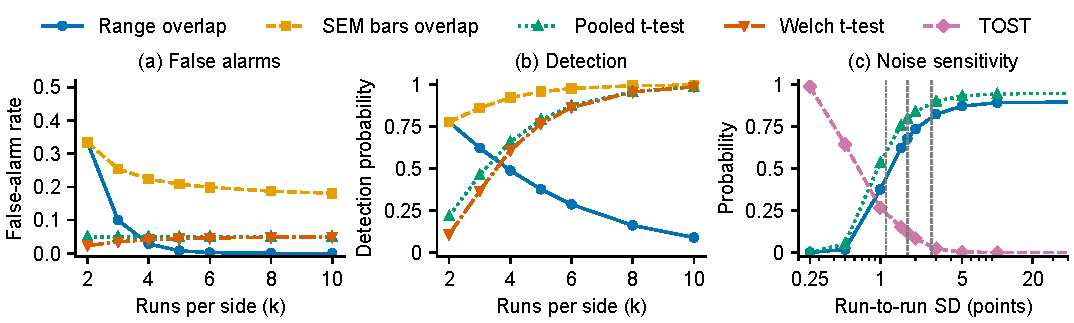
\includegraphics[width=\textwidth]{figures/fig1_rules.pdf}
\caption{Normal run-to-run noise; $k$ is runs per side. (a) False-alarm rate against $k$. (b) Detection of a fixed 2 SD gap against $k$. (c) A true gap of 2 points at $k=3$ against the run-to-run SD: the probability that range overlap passes, that a pooled $t$-test finds no significant gap, and that TOST shows equivalence within 3 points; dashed lines mark the SD quartiles of the published runs.}
\label{fig:rules}
\end{figure*}

\textbf{Realistic noise.} Repeating the analysis with run scores built from the per-task pass probabilities of 30 adapters (Section~\ref{sec:rq3}) leaves the ordering unchanged; with ties the overlap rule's median false alarm is 0.07, and a 5-point loss is caught 0.58 of the time by range overlap and 0.47 by the pooled $t$-test.

\textbf{What a pass means.} A pass is a failure to reject at the 10\% level with a difference test. It never means that the port is within any stated distance of the original: under a perfect port with $k=3$ the smallest margin within which equivalence can be shown is 2.3 run SDs on average, about 3.9 points at the median SD. The paper's wordings describe stricter checks than the guide's rule, not laxer ones: read literally they flag 25 to 44\% of perfect ports (Table~\ref{tab:rules}).

\section{RQ2: What the published runs establish}
\label{sec:rq2}

\textbf{Method.} We built one comparison per experiment under a rule written down before the analysis: which metric row is the main one (the row matching the paper's tables, else the headline metric, else the first point-scale row), which rows are excluded, and how units are handled. Six amendments were logged with date and reason; the three that touch the rule leave the headline count unchanged. For each comparison we computed the gap (Harbor minus original), the pooled-$t$ 90\% confidence interval, and the \emph{smallest provable margin}: the distance from zero to the farther end of that interval. Equivalence within $\pm m$ is shown when the whole 90\% interval lies inside $\pm m$, the two-one-sided-tests (TOST) procedure at the 5\% level~\cite{schuirmann_1987,lakens_2017}.

\textbf{Results.} The ports look close. Over the 58 comparisons the median absolute gap is 0.67 points, the median run-to-run SD is 1.71 points, and no gap is distinguishable from zero at the 95\% level. The evidence that they are close is thin: the quartiles of the smallest provable margin are 2.4, 4.4 and 6.0 points. Equivalence within 2, 3 and 5 points can be shown for 7, 22 and 36 of the 58, and one in four cannot show it even within 6 points (Fig.~\ref{fig:margins}).

\begin{figure}[t]
\centering
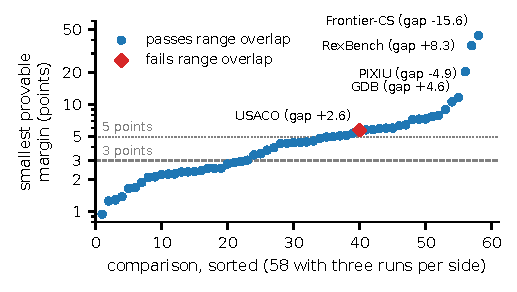
\includegraphics[width=\columnwidth]{figures/fig2_margins.pdf}
\caption{Smallest margin within which each of the 58 published comparisons can show equivalence (TOST, 90\% interval), sorted. Lines mark 3 and 5 points. The one comparison that fails range overlap, USACO, sits in the middle; the four largest gaps all pass.}
\label{fig:margins}
\end{figure}

\textbf{The rule's verdicts.} Fifty-seven comparisons pass range overlap; 21 of them cannot show equivalence within 5 points and 35 cannot within 3. The rule passes the four largest gaps: Frontier-CS at $-15.6$ points (a 10-task subset with a run SD of 16 points), RexBench at $+8.3$, PIXIU at $-4.9$ and GDB at $+4.6$, whose smallest provable margins are 44, 35, 20 and 12 points. The one failure, USACO, misses overlap by 0.1 point and has a smallest provable margin of 5.8 points, which 18 of the 57 passes exceed. The paper's SEM wordings would have failed 4, 12 and 18 of the 58 under readings S1, S2 and S3.

\textbf{Selection.} If all 58 ports were perfect and runs independent, range overlap would flag 5.8 of them on average; it flagged one (binomial lower tail 0.017). This is what the process implies: non-overlap is treated as an error to be fixed and rerun, so the records that reach the repository are the ones that ended up passing. Published pass rates therefore cannot validate the rule, and the rates of Section~\ref{sec:rq1} are properties of the rule under stated noise models, not of the published ports.

\textbf{Stability.} Counts at fixed margins are knife-edge: shifting every margin by 0.1 point moves the within-5 count between 34 and 37, and Welch intervals lower it from 36 to 31; the quartiles are the stable summary. Comparisons run on a subset of tasks (22 of the 58) are noisier than full-set ones, with a median run SD of 2.3 against 1.5 points.

\section{RQ3: A better check and its cost}
\label{sec:rq3}

\textbf{Runs.} Table~\ref{tab:runs} gives the runs per side an equivalence test needs for 80\% power at the SD quartiles observed in the 58 comparisons (1.1, 1.7 and 2.7 points), for margins of 2, 3 and 5 points, under a true gap of 0 and of 0.6 points (about the observed median). At the median noise a 3-point margin needs about 7 runs per side; per comparison with its own SD the median need is 7 (quartiles 4 to 16), and two comparisons would need more than 400. The plug-in rule ``run until the interval fits'' has only 12 to 78\% power across this table.

\begin{table}[t]
\caption{Runs per side for 80\% power to show equivalence within $\pm m$ points at the observed SD quartiles, for a true gap of 0 (and of 0.6 points).}
\label{tab:runs}
\centering
\begin{tabular}{lccc}
\toprule
margin & SD 1.1 & SD 1.7 & SD 2.7 \\
\midrule
$\pm2$ & 7 (9) & 14 (20) & 33 (49) \\
$\pm3$ & 4 (4) & 7 (8) & 16 (18) \\
$\pm5$ & 3 (3) & 3 (4) & 6 (7) \\
\bottomrule
\end{tabular}

\end{table}

\textbf{Per-task outcomes.} Both sides already produce per-task results, and the guide's debugging playbook asks for a per-task split~\cite{harbor_contributing}. We recovered them from the published files for 44 adapters with both sides; 27 meet our inclusion rule (replicate runs of one experiment, at least 20 shared tasks, and files that reproduce the published run scores or carry a documented exception). Pairing the sides task by task does not tighten the interval for the gap. Under shared per-task pass probabilities the paired interval should be about a sixth narrower than the run-level one, only because the latter must estimate its noise from three numbers; in fact it is wider in 15 of 26 adapters. The reason is that the two sides disagree on individual tasks more than shared pass probabilities allow in 14 of 27 adapters, even though the mean gap is exchangeable in all 27 and a stratified-by-task test rejects for none of the 21 adapters with binary outcomes. Some tasks pass in every run on one side and fail in every run on the other (13 in DS-1000). Run scores cannot show this, and one pair of sides cannot say whether it comes from the port or from side-specific effects such as seeds, environments or caching.

The files also show that in 9 of the 30 adapters with binary outcomes and validated replicate Harbor runs, the between-run variance of the published Harbor run scores is below a tenth of what their own within-task flip rates imply under independent outcomes (dispersion-ratio quartiles 0.10, 0.52, 1.26). FinanceAgent, for example, reports 40 of 50 passes in each of three runs while individual tasks flip between runs. Either outcomes within a run are negatively dependent across tasks or the runs are not independent replicates; we report it as an open data-quality question.

\textbf{Injected defects.} To compare tests on realistic data we simulated both sides from the per-task pass probabilities of the same 30 adapters, with a defect that breaks (always fails) or leaks (always passes) a fraction of tasks on the port side, 2{,}000 replications per cell (Fig.~\ref{fig:defects}). With three runs, a defect that breaks 10\% of tasks (a loss of 5.4 points on average) is caught by range overlap 0.64 of the time, at a false-alarm rate of 0.07 under this model; by the pooled $t$-test 0.59; by the stratified-by-task test (Cochran-Mantel-Haenszel; McNemar at one run) 0.67; and by a paired $t$-test on per-task differences 0.54, the last three at 0.05. The paired $t$ is the wrong paired statistic for a sparse defect: its standard error absorbs the between-task spread of the defect itself, which does not shrink with runs. With ten runs the pooled $t$ and the stratified test catch the same defect 0.86 of the time, the paired $t$ 0.67, and range overlap 0.36. A perfect port is shown equivalent within 5 points 0.51 of the time at $k=3$, 0.75 at $k=5$ and 0.94 at $k=10$. The 21 well-dispersed adapters give the same picture; a flat Beta(1,1) prior on pass probabilities lowers every rate by about a third; resampling the 8 fractional-score adapters' observed rewards gives 0.72, 0.67 and 0.59 for range overlap, pooled $t$ and paired $t$.

\begin{figure*}[t]
\centering
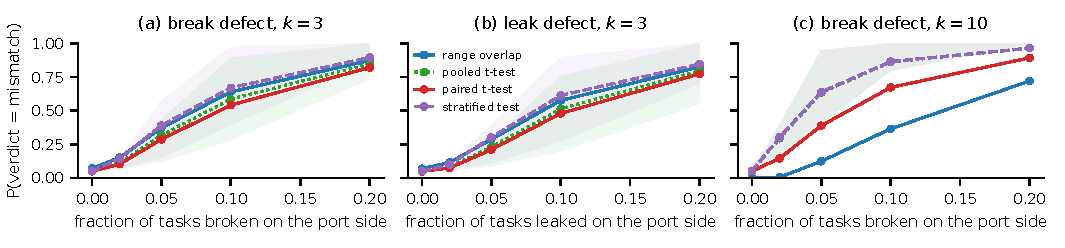
\includegraphics[width=\textwidth]{figures/fig3_defects.pdf}
\caption{Detection of injected defects, mean over 30 adapters simulated from their published per-task outcomes: (a) break defects at $k=3$, (b) leak defects at $k=3$, (c) break defects at $k=10$. Bands: interquartile range across adapters for the pooled $t$ and stratified tests. The value at zero is the false-alarm rate.}
\label{fig:defects}
\end{figure*}

\textbf{A verdict tool.} A script in our repository reads any \texttt{parity\_experiment.json} and prints the overlap verdict, the gap with its interval, the smallest provable margin, and the runs per side needed for 80\% power at that row's own noise. For USACO: gap $+2.6$ [$-1.4$, $+6.7$], margin 5.8 points, 7 runs for $\pm 3$. For RexBench: gap $+8.3$ [$-27$, $+44$], margin 35 points, 464 runs.

\section{Recommended protocol}

\begin{enumerate}
\item State the margin before running: how many points of difference would make the port a different benchmark. For most scores 3 to 5 points; tighter near a decision threshold.
\item Choose the run count from the noise: enough runs per side for 80\% power at that margin (Table~\ref{tab:runs}). When the noise is unknown, start with at least five and add runs once the first runs show it.
\item Report the gap with its 90\% interval and the smallest provable margin. Declare ``equivalent within $\pm m$'' only when the interval lies inside $\pm m$; otherwise ``not yet shown'', which asks for runs, not for a rewrite.
\item Publish per-task outcomes on both sides with aligned task ids, report a stratified-by-task test, and investigate tasks that differ in every run.
\item Keep range overlap as a sanity check at most.
\end{enumerate}
The cost is about seven runs per side instead of three at the observed noise for a 3-point margin, and a reporting change.

\section{Threats to validity}

\emph{Noise models.} We treat run scores as independent draws with a common variance and check the conclusions under binomial and per-task models; all three rank the rules the same way. Run-level shocks such as infrastructure noise~\cite{segato_infra_noise} are not modelled. \emph{Selection.} The published ports are post-selection, so their pass rates cannot validate any rule; our rates are model properties. \emph{Few runs.} Three runs give a noisy SD; we report pooled quartiles and use per-task data as a second estimate. \emph{Metric rule.} The main-metric rule and its amendments are a choice; the three that touch the rule leave the within-5 count unchanged, a 0.1-point shift moves it between 34 and 37, and Welch intervals give 31. Metrics of different kinds (pass rates, F1, rewards) sit on one point scale; subsets are noisier than full sets. \emph{Per-task data.} They come in one format per adapter, validated only against the published run scores; 13 of the 44 two-sided folders are excluded and 6 of the 27 used carry documented exceptions. The per-task model's prior changes detection rates by up to a factor of two, and the model assumes independent outcomes within a run, so run-level rates are understated for the under-dispersed adapters. \emph{Snapshot.} One commit on one day of a moving repository; we reran no benchmark.

\section{Related work}

That overlap of error bars or intervals is a poorly calibrated test is classical~\cite{schenker_gentleman_2001,payton_2003,belia_2005}, and the quantity the rule inspects, whether one sample's extremes clear the other's, is the one Tukey's quick two-sample test counts~\cite{tukey_1959}. Equivalence testing with a stated margin is standard in other fields~\cite{schuirmann_1987,lakens_2017}, and absence of evidence is not evidence of absence~\cite{altman_bland_1995}. Noise in language-model and agent evaluation has been quantified with error bars, clustering and variance decomposition~\cite{miller_error_bars,hardy_reliability,segato_infra_noise}; re-implementations of the same benchmark are known to drift~\cite{biderman_lessons,pimentel_beyond_metrics,uniace}, and other ecosystems accept re-implementations with a fixed tolerance or a test against a reference distribution~\cite{inspect_evals,mlperf_training_rules}. Recent work applies paired tests and TOST to claims of equivalence between models, scaffolds or compressed variants~\cite{liu_han_harness,singh_compressed,liu_converged}; Zhang \emph{et al.} make the same gate-versus-certificate point for release decisions~\cite{zhang_upgrades}. Inside Harbor, a few adapter records already report $t$-tests, permutation tests or per-task agreement, a proposed tool offers a paired permutation test~\cite{harbor_pr_517}, and one port that had passed parity later proved to leak gold tests~\cite{harbor_issue_1067}. None of this work analyses the acceptance rule itself, asks what the published parity runs can establish, or costs the fix.

\section{Conclusion}

A parity experiment under the range-overlap rule proves that a difference test with a 10\% false-alarm rate did not fire. It cannot show that a port is within any stated distance of the original, and the published runs can show equivalence within 5 points for about six ports in ten. The fix is cheap: a margin, about seven runs per side, an equivalence test, and the per-task outcomes both sides already have.

\section*{Acknowledgments}
We thank the Harbor maintainers, whose published runs and per-task files made this analysis possible. AI assistance: to be written by the authors.

\bibliographystyle{IEEEtran}
\bibliography{refs}

\end{document}
